\documentclass[cn,12pt,founder,a4paper]{elegantpaper}
\usepackage{listings,color}

% Matlab highlight color settings
\definecolor{mKeyword}{RGB}{0,0,255}          % bule
\definecolor{mString}{RGB}{160,32,240}        % purple
\definecolor{mComment}{RGB}{34,139,34}        % green
\definecolor{mBackground}{RGB}{245,245,245}   % lightgrey
\definecolor{mNumber}{RGB}{134,145,148}       % gray
\definecolor{Numberbg}{RGB}{237,240,241}      % lightgrey

% Python highlight color settings
\definecolor{pKeyword}{RGB}{228,0,128}        % magenta
\definecolor{pString}{RGB}{148,0,209}         % purple
\definecolor{pComment}{RGB}{117,113,94}       % gray
\definecolor{pIdentifier}{RGB}{166, 226, 46}  %
\definecolor{pBackground}{RGB}{245,245,245}   % lightgrey
\definecolor{pNumber}{RGB}{134,145,148}       % gray

\lstnewenvironment{Matlab}{
\lstset{language=Matlab,                     
  xleftmargin=30pt,
  xrightmargin=10pt,
  frame=l,
  framesep=15pt,
  basicstyle=\footnotesize\fontspec{Consolas},
  keywordstyle={\color{mKeyword}},     % sets color for keywords
  stringstyle={\color{mString}},       % sets color for strings
  commentstyle={\color{mComment}},     % sets color for comments
  backgroundcolor=\color{mBackground}, % choose the background color
  keywords={break,case,catch,classdef,continue,else,elseif,end,for,
  function,global,if,otherwise,parfor,persistent,return,spmd,switch,try,while},
  showspaces=false,                    % show spaces adding particular underscores
  showstringspaces=false,              % underline spaces within strings
  showtabs=false,                      % show tabs within strings adding particular underscores
  tabsize=4,                           % sets default tabsize to 2 spaces
  captionpos=t,                        % sets the caption-position to bottom
  breaklines=true,                     % sets automatic line breaking
  framexleftmargin=5pt,
  fillcolor=\color{Numberbg},
  rulecolor=\color{Numberbg},
  numberstyle=\tiny\color{mNumber},
  numbersep=9pt,                       % how far the line-numbers are from the code
  numbers=left,                        % where to put the line-numbers
  stepnumber=1,                        % the step between two line-numbers.
}}{\lstname}

\lstnewenvironment{Python}{
\lstset{language=python,               
  xleftmargin=30pt,
  xrightmargin=10pt,
  frame=l,
  framesep=15pt,
  basicstyle=\footnotesize\fontspec{SourceCodePro-Regular},
  keywordstyle=\color{pKeyword},       % sets color for keywords
  stringstyle=\color{pString},         % sets color for strings
  commentstyle=\color{pComment},       % sets color for comments
  backgroundcolor=\color{pBackground}, % choose the background color
  emph={format_string,eff_ana_bf,permute,eff_ana_btr},
  emphstyle=\color{pIdentifier}
  showspaces=false,                    % show spaces adding particular underscores
  showstringspaces=false,              % underline spaces within strings
  showtabs=false,                      % show tabs within strings adding particular underscores
  tabsize=4,                           % sets default tabsize to 2 spaces
  captionpos=t,                        % sets the caption-position to bottom
  breaklines=true,                     % sets automatic line breaking
  framexleftmargin=5pt,
  fillcolor=\color{Numberbg},
  rulecolor=\color{Numberbg},
  numberstyle=\tiny\color{pNumber},
  numbersep=9pt,                       % how far the line-numbers are from the code
  numbers=left,                        % where to put the line-numbers
  stepnumber=1,                        % the step between two line-numbers.
}}{}
\usepackage{silence}                                             
\WarningsOff* 
\usepackage{amsmath,amscd,amssymb,amsthm,amsfonts}  
\usepackage{extarrows}
\usepackage{mathtools}
\usepackage{nicematrix}
\usepackage{booktabs}
\usepackage{makecell}
\usepackage{float}
\usepackage{subfigure}
\usepackage[most]{tcolorbox}
\colorlet{LightLavender}{red!30!}
\tcbset{
  on line, left=0pt, right=0pt, top=0pt, bottom=0pt,
  colframe=white, colback=LightLavender, fontupper=\fontspec{Consolas},
  highlight math style={enhanced}
}
\hypersetup{pdftitle=非线性方程组的牛顿迭代法,pdfauthor=李徐瑾,pdfkeywords=电子科技大学}
\let\Bbbk\undefined
\let\heavymath\undefined
\usepackage[complete,subscriptcorrection,slantedGreek]{mtpro2} 

\newcommand*{\bbR}{\mathbb{R}}
\newcommand*{\transpose}{\mathrm{T}}
\newcommand*{\exist}{\exists\mathop{}\!}
\newcommand*{\douprime}{{\prime\prime}}
\newcommand*{\gt}[1]{\CJKfontspec{GuoTi-Regular}#1}
\newcommand*{\J}{\b{\mathrm{J}}}
\newcommand*{\e}{\mathrm{e}}
\renewcommand*{\H}{\b{\mathrm{H}}}
\renewcommand*{\emph}[1]{{\heiti{#1}}}
\renewcommand*{\b}{\boldsymbol}
\renewcommand{\thetable}{\thesection{}.\arabic{table}}
\renewcommand{\thefigure}{\thesection{}.\arabic{figure}}
\renewcommand{\theequation}{\thesection{}.\arabic{equation}}
\DeclareMathOperator*{\st}{s.t.}

\title{非线性方程组的牛顿迭代法}
\author{\kaishu 姓名: 李徐瑾\\ \kaishu 学号: 202021110109\qquad 序号: 66}
\date{\zhtoday}
\institute{\gt 电子科技大学数学科学学院}


\begin{document}

\maketitle

\begin{abstract}
非线性方程组在实际问题中经常出现,并且在科学计算中的地位越来越重要,很多常见的线性模型都是在一定条件下由非线性问题简化得到的,为了得到更符合实际的解答,往往需要直接研究非线性模型,然而从线性到非线性是一个质的飞跃,方程的性质不同,所使用的求解方法也有很大的差别,本文主要先给出由非线性方程到一般非线性方程组牛顿迭代法的分析及推导过程,而后使用牛顿迭代法求解非线性方程组\eqref{eq:11},并给出由M{\footnotesize{ATLAB}}编程分析实现的过程. 
\keywords{非线性方程组,牛顿迭代法,雅可比矩阵,M{\footnotesize{ATLAB}}}
\end{abstract}

\section{非线性方程组与牛顿迭代法}

\subsection{非线性方程组}
非线性方程组是非线性科学的重要组成部分.\par
考虑方程组
\begin{equation}\label{eq:1}
  \begin{cases}
    f_1(x_1,x_2,\cdots,x_n)=0,\\
    f_2(x_1,x_2,\cdots,x_n)=0,\\
    \hspace*{3.5em}\vdots\\
    f_n(x_1,x_2,\cdots,x_n)=0.
  \end{cases}
\end{equation}
其中\(f_1,f_2,\cdots,f_n\)均是\(x_1,x_2,\cdots,x_n\)的多元函数.\par 
如果采用向量记法\(\b{x}=(x_1,x_2,\cdots,x_n)^\transpose\in\bbR^n,\b{F}=(f_1,f_2,\cdots,f_n)^\transpose\),方程组\eqref{eq:1}可表示为
\begin{equation}\label{eq:2}
  \b{F}(\b{x})=\b{0}.
\end{equation}
当\(n\geqslant 2\)且\(f_i(i=1,2,\cdots,n)\)中至少有一个是自变量\(x_i(i=1,2,\cdots,n)\)的非线性函数时,则称方程组\eqref{eq:1}为\emph{非线性方程组}.\par
非线性方程组\eqref{eq:1}的求解无论是在理论还是在实际解法上均比线性方程组和单个方程的求解要复杂和困难,可能无解也可能有一个或者多个解.\par
求方程组\eqref{eq:1}的根可直接将单个方程\((n=1)\)的求解方法加以推广,实际上只要把单变量函数\(f(x)\)看成向量函数\(\b{F}(\b{x})\),将方程组\eqref{eq:1}改写成方程组\eqref{eq:2},就可将之前讨论的求根方法用于求解方程组\eqref{eq:2}的根,假设向量函数\(\b{F}(\b{x})\)是定义在区域\(D\subset\bbR^n\),若对于\(\b{x}_0\in D\),有
\[\lim_{\b{x}\to\b{x}_0}\b{F}(\b{x})=\b{F}(\b{x}_0),\]
则称\(\b{F}(\b{x})\)在\(\b{x}_0\)处\emph{连续},即\(\forall\varepsilon>0,\exist\delta>0\),当\(0<\Vert\b{x}-\b{x}_0\Vert<\delta\)时,使得
\[\Vert\b{F}(\b{x})-\b{F}(\b{x}_0)\Vert<\varepsilon.\]
如果\(\b{F}(\b{x})\)在\(D\)上的每一点均连续,则称\(\b{F}(\b{x})\)在域\(D\)中连续.\par
向量函数\(\b{F}(\b{x})\)的导数\(\b{F}^\prime(\b{x})\)称为\(\b{F}\)的\emph{雅克比矩阵},通常记为\(\J(\b{x})\),即
\begin{equation}\label{eq:3}
  \J(\b{x})\coloneqq\b{F}^\prime(\b{x})=
  \begin{bmatrix}
    \frac{\partial f_1(x)}{\partial x_1}&\frac{\partial f_1(x)}{\partial x_2}&\cdots&\frac{\partial f_1(x)}{\partial x_n}\\[2pt]
    \frac{\partial f_2(x)}{\partial x_1}&\frac{\partial f_2(x)}{\partial x_2}&\cdots&\frac{\partial f_2(x)}{\partial x_n}\\[2pt]
    \vdots&\vdots&\ddots&\vdots\\[2pt]
    \frac{\partial f_n(x)}{\partial x_1}&\frac{\partial f_n(x)}{\partial x_2}&\cdots&\frac{\partial f_n(x)}{\partial x_n}
  \end{bmatrix}.
\end{equation}

\subsection{牛顿迭代法}
事实上,将单个方程的牛顿迭代法直接用于方程组\eqref{eq:2},则可得到解非线性方程组的牛顿迭代法,因此我们先分析非线性方程的数值解法,然后再将其延伸到方程组的解法.

\subsubsection{牛顿迭代法的思想}
牛顿迭代法实质上是一种线性化方法,基本思想是将非线性方程\(f(x)=0\)逐步归结为某种线性方程来求解.\par
设已知方程\(f(x)=0\)有近似根\(x_k(f^\prime(x_k)\ne 0)\),将函数\(f(x)\)在点\(x_k\)展开,则有
\[f(x)\approx f(x_k)+f^\prime(x_k)(x-x_k),\]
于是方程\(f(x)=0\)可近似地表示为
\[f(x_k)-f^\prime(x_k)(x-x_k)=0.\]
这是一个线性方程,记其根为\(x_{k+1}\),则\(x_{k+1}\)的计算公式为
\begin{equation}\label{eq:4}
  x_{k+1}=x_k-\frac{f(x_k)}{f^\prime(x_k)},\quad k=0,1,\cdots.
\end{equation}
这便是\emph{牛顿迭代法},亦称为\emph{切线法}.\par
关于牛顿迭代法的收敛性,根据式\eqref{eq:4}知迭代公式为
\[\varphi(x)=x-\frac{f(x)}{f^\prime(x)},\]
因此
\[\varphi^\prime(x)=\frac{f(x)f^\douprime(x)}{[f^\prime(x)]^2}.\]
假设\(x^\star\)是\(f(x)\)的单根,即\(f(x^\star)=0,f^\prime(x^\star)\ne 0\),故牛顿迭代法是平方收敛的. 即
\[\lim_{k\to\infty}\frac{x_{k+1}-x^\star}{(x_k-x^\star)^2}=\frac{f^\douprime(x^\star)}{2f^\prime(x^\star)}.\]\par
牛顿迭代法有明显的几何意义,方程\(f(x)=0\)的根\(x^\star\)可解释为曲线\(y=f(x)\)与\(x\)轴交点的横坐标,即
\begin{figure}[h]
  \centering
  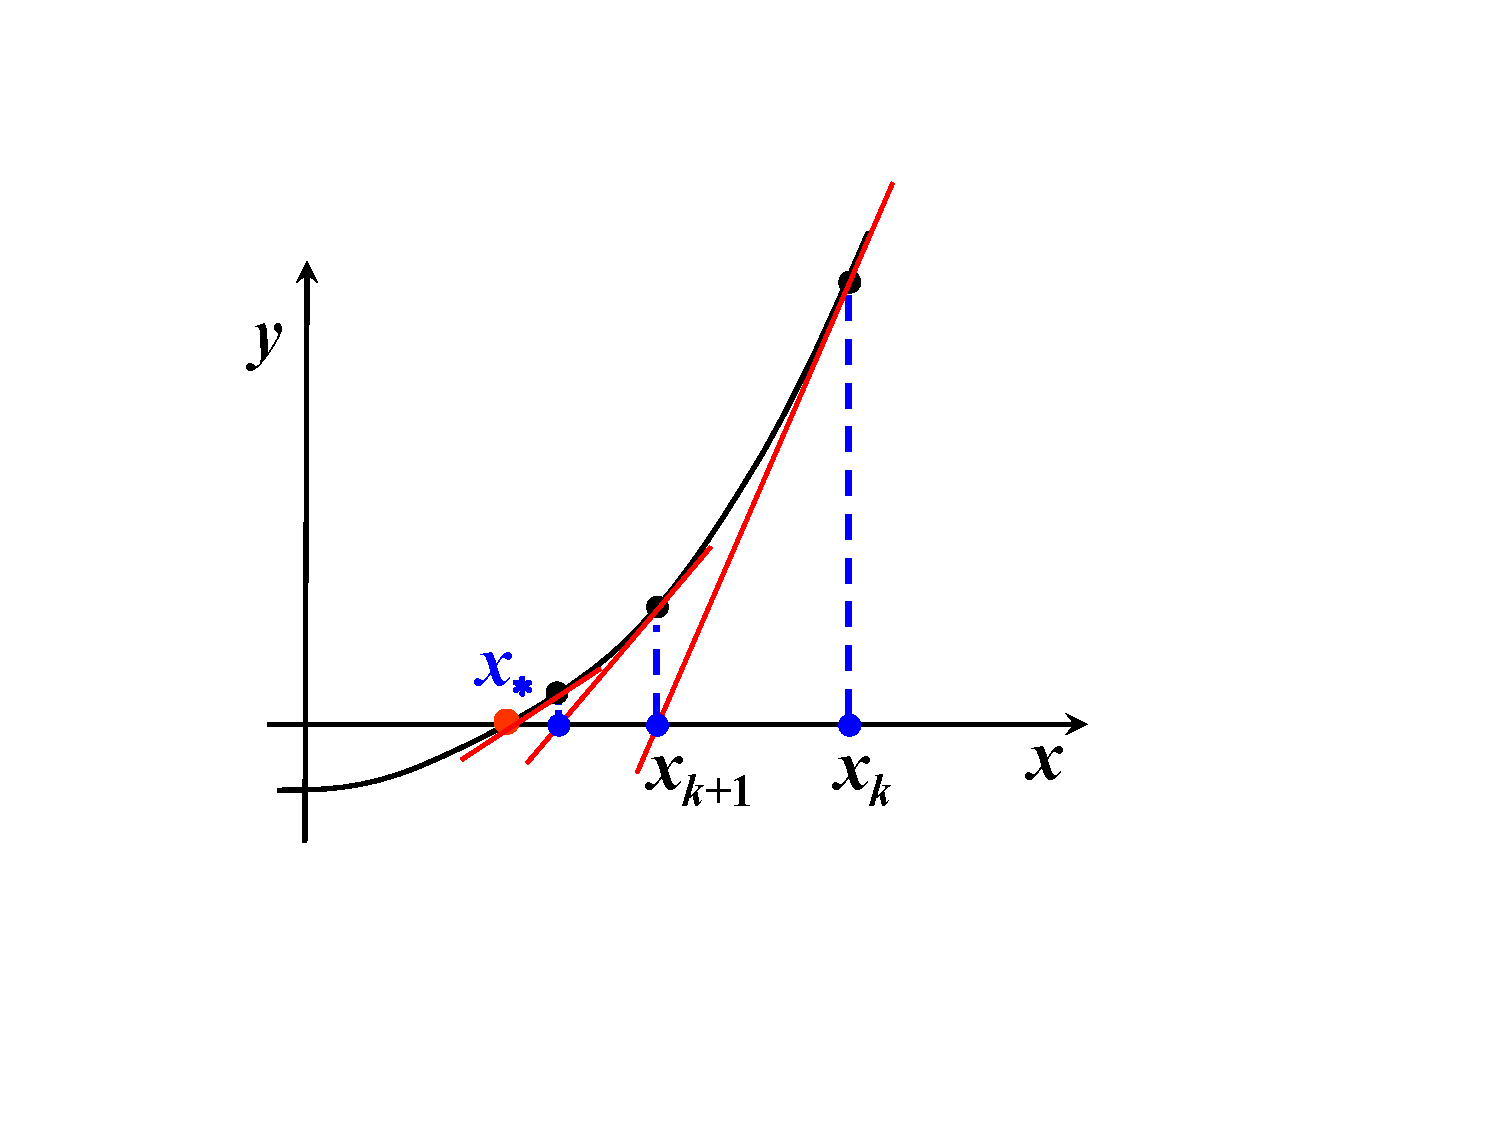
\includegraphics[scale=0.55]{image/Newton.pdf}
  \caption{牛顿迭代法的几何意义}
\end{figure}
\begin{theorem}\label{th:1}
  若\(f(x)\)在\(x^\star\)的某邻域内具有连续的二阶导数,且满足\(f(x^\star)=0,f^\prime(x^\star)\ne 0\),则对充分靠近\(x^\star\)的初始值\(x_0\),牛顿迭代法生成的序列\(\lbrace x_n\rbrace\)至少平方收敛于\(x^\star\).
\end{theorem}
\begin{theorem}[非局部收敛定理]\label{th:2}
  给定方程\(f(x)=0\),如果函数\(f(x)\in C^2[a,b]\)且满足:
  \begin{enumerate}
    \item[(1)] \(f(a)f(b)<0\),
    \item[(2)] \(f^\prime(x),f^\douprime(x)\)在\([a,b]\)上连续且不变号,
    \item[(3)] \(\exist x_0\in[a,b],\st f(x_0)f^\douprime(x_0)>0\).   
  \end{enumerate}
  则方程\(f(x)=0\)在\([a,b]\)上有唯一的根\(x^\star\).
\end{theorem}
现在我们可将牛顿迭代法的思想归结为下列的步骤:
\begin{enumerate}
  \item[\emph{步一}] 任取迭代初始值\(x_0\);
  \item[\emph{步二}] 计算\(x_1=x_0-{f(x_0)}/{f^\prime(x_0)}\);
  \item[\emph{步三}] 判断收敛性,若\(\vert x_1-x_0\vert<\varepsilon\)或\(\vert f(x_0)\vert<\varepsilon\),则算法收敛,停止计算,输出近似解\(x_1\);
  \item[\emph{步四}] 令\(x_0\leftarrow x_1\),返回\emph{步二}.   
\end{enumerate}

\subsubsection{牛顿迭代法的改进}
我们已经知道牛顿迭代法是平方收敛的,因而其优点是收敛快. 但缺点也较为明显,主要表现为以下两点:
\begin{itemize}
  \item 每一步迭代均需要计算\(f(x_k),f^\prime(x_k)\)且有时\(f^\prime(x_k)\)计算量偏大,
  \item 初始值\(x_0\)仅在根\(x^\star\)附近才能保证收敛,选取不恰当的初始值可能导致不收敛.
\end{itemize}\par
为了克服上述两个缺点,我们通常可以采用\emph{简化牛顿法}和\emph{牛顿下山法}.
\begin{enumerate}
  \item[(1)] \emph{简化牛顿法}的迭代公式为
  \begin{equation}\label{eq:5}
    x_{k-1}=x_k-Cf(x_k),\quad C\ne 0,k=0,1,\cdots.
  \end{equation}  
  迭代函数\(\varphi(x)=x-Cf(x)\).\par
  若\(\vert\varphi^\prime(x)\vert=\vert 1-Cf^\prime(x)\vert<1\),即当\(0<Cf^\prime(x)<2\)时,在根\(x^\star\)附近成立,此时迭代公式\eqref{eq:5}\emph{局部收敛}. 若取\(C={1}/{f^\prime(x_0)}\),则称为\emph{简化牛顿法},此方法的几何意义是用斜率为\(f^\prime(x_0)\)的平行弦与\(x\)轴的交点作为\(x^\star\)的近似,因此亦称为\emph{平行弦法},此种方法计算量相对较小,但只是线性收敛.
  \item[(2)] \emph{牛顿下山法}的收敛性依赖于初始值\(x_0\)的选取,如果\(x_0\)偏离根\(x^\star\)较远,则可能导致发散.
  \emph{下山法}意即对迭代过程添加附加条件
  \[\vert f(x_{k+1})\vert<\vert f(x_k)\vert.\]
  将下山法与牛顿法结合,以此在保证函数值稳定下降的前提下加快牛顿法的收敛速度. 牛顿下山法的迭代公式为
  \[x_{k+1}=x_k-\lambda\frac{f(x_k)}{f^\prime(x_k)},\quad k=0,1,\cdots.\]
  其中\(\lambda(0<\lambda\leqslant 1)\)称为\emph{下山因子}.
\end{enumerate}\par
接下来我们考虑重根的情形,即当方程\(f(x)=0\)有\(m\)重根时,有
\[f(x^\star)=f^\prime(x^\star)=\cdots=f^{(k-1)}(x^\star)=0,\quad f^{(m)}(x^\star)\ne 0.\]
只有\(f^\prime(x_k)\ne 0\)仍可使用牛顿迭代法公式\eqref{eq:4}计算. 此时迭代函数的导数满足
\[\varphi^\prime(x^\star)=1-\frac{1}{m},\quad\vert\varphi^\prime(x^\star)\vert<1.\]
故牛顿迭代法求重根只是线性收敛的. 不妨取
\[\varphi(x)=x-m\frac{f(x)}{f^\prime(x)},\]
则\(\varphi^\prime(x^\star)=0\). 采用迭代公式
\[x_{k+1}=x_k-m\frac{f(x_k)}{f^\prime(x_k)},\quad k=0,1,\cdots.\]
这是二阶收敛的,但我们需要求出\(x^\star\)的重数\(m\).\par
不妨令\(\mu(x)={f(x)}/{f^\prime(x)}\),如果\(x^\star\)是\(f(x)=0\)的\(m\)重根,则
\[\mu(x)=\frac{(x-x^\star)g(x)}{mg(x)\mid(x-x^\star)g^\prime(x)},\]
故\(x^\star\)是\(\mu(x)=0\)的单根,因而可构造迭代函数
\[x_{k+1}=x_k-\frac{f(x_k)f^\prime(x_k)}{[f^\prime(x_k)]^2-f(x_k)f^\douprime(x_k)},\quad k=0,1,\cdots.\]

\subsubsection{二元非线性方程组牛顿迭代法的推导}
现在我们考虑二元非线性方程组
\begin{equation}\label{eq:6}
  \begin{cases}
    f(x,y)=0,\\
    g(x,y)=0.
  \end{cases}
\end{equation}
的迭代的方程,我们先给出\emph{一元函数的Taylor公式}和\emph{二元函数的Taylor公式}.
\begin{theorem}[一元函数的Taylor公式]\label{th:3}
  若函数\(f(x)\)在含有\(x_0\)的某开区间\((a,b)\)内具有直至\((n+1)\)阶的导数,则对任一\(x\in(a,b)\),有
  \[f(x)=f(x_0)+f^\prime(x_0)(x-x_0)+\frac{f^\douprime(x_0)}{2!}(x-x_0)^2+\cdots+\frac{f^{(n)}(x_0)}{n!}(x-x_0)^n+R_n(x).\]
  其中\(R_n(x)=\frac{f^{(n+1)}(\xi)}{(n+1)!}(x-x_0)^{n+1},\xi\in(x_0,x)\).
\end{theorem}
\begin{theorem}[二元函数的Taylor公式]\label{th:4}
  设\(z=f(x,y)\)在点\((x_0,y_0)\)的某邻域内连续且有直至\((n+1)\)阶的连续偏导数,\((x_0+h,y_0+h)\)为此邻域内任意一点,则有
  \begin{align*}
    f(x_0+h,y_0+h)&=f(x_0,y_0)+\Big(h\frac{\partial}{\partial x}+k\frac{\partial}{\partial y}\Big)f(x_0,y_0)\\
    &+\frac{1}{2!}\Big(h\frac{\partial}{\partial x}+k\frac{\partial}{\partial y}\Big)^2 f(x_0,y_0)+\cdots+\frac{1}{n!}\Big(h\frac{\partial}{\partial x}+k\frac{\partial}{\partial y}\Big)^n f(x_0,y_0)\\
    &+\frac{1}{(n+1)!}\Big(h\frac{\partial}{\partial x}+k\frac{\partial}{\partial y}\Big)^{n+1}f(x_0+\theta h,y_0+\theta k),\quad\theta\in(0,1).
  \end{align*}
  其中
  \[\Big(h\frac{\partial}{\partial x}+k\frac{\partial}{\partial y}\Big)^m f(x_0,y_0)=\sum_{p=0}^{m}\binom{m}{p}h^pk^{m-p}\frac{\partial^m f}{\partial x^p\partial y^{m-p}}\Bigg\vert_{(x_0,y_0)}.\]
\end{theorem}\par
接下来我们来推导二元函数\eqref{eq:6}的牛顿迭代法,假设\(z=f(x,y)\)在点\((x_0,y_0)\)的某邻域内连续且有直至\(2\)阶的连续偏导数,\((x_0+h,y_0+k)\)为此邻域内任意一点,则有
\begin{align*}
  f(x_0+h,y_0+k)&\approx f(x_0,y_0)\\
  &+\Big(h\frac{\partial}{\partial x}f(x,y)\Big\vert_{x=x_0}+k\frac{\partial}{\partial y}f(x,y)\Big\vert_{y=y_0}\Big),\quad h=x-x_0,k=y-y_0.
\end{align*}\par
于是方程\(f(x,y)=0\)可近似的表示为
\[f(x_k,y_k)+\Big(h\frac{\partial}{\partial x}f(x,y)\Big\vert_{x=x_k}+k\frac{\partial}{\partial y}f(x,y)\Big\vert_{y=y_k}\Big)=0,\]
即\(f(x_k,y_k)+(x-x_k)f_k(x_k,y_k)+(y-y_k)f_y(x_k,y_k)=0\).\par
同理设\(z=g(x,y)\)在点\((x_0,y_0)\)的某邻域内连续且有直至\(2\)阶的连续偏导数,\((x_0+h,y_0+k)\)为此邻域内任意一点,则有
\begin{align*}
  g(x_0+h,y_0+k)&\approx g(x_0,y_0)\\
  &+\Big(h\frac{\partial}{\partial x}g(x,y)\Big\vert_{x=x_0}+k\frac{\partial}{\partial y}g(x,y)\Big\vert_{y=y_0}\Big),\quad h=x-x_0,k=y-y_0.
\end{align*}\par
于是方程\(g(x,y)=0\)可近似的表示为
\[g(x_k,y_k)+\Big(h\frac{\partial}{\partial x}g(x,y)\Big\vert_{x=x_k}+k\frac{\partial}{\partial y}g(x,y)\Big\vert_{y=y_k}\Big)=0,\]
即\(g(x_k,y_k)+(x-x_k)g_k(x_k,y_k)+(y-y_k)g_y(x_k,y_k)=0\).\par
于是得到方程组
\begin{equation}\label{eq:7}
  \begin{cases}
    f(x_k,y_k)+(x-x_k)f_k(x_k,y_k)+(y-y_k)f_y(x_k,y_k)=0,\\
    g(x_k,y_k)+(x-x_k)g_k(x_k,y_k)+(y-y_k)g_y(x_k,y_k)=0.
  \end{cases}
\end{equation}\par
接下来我们求解方程组\eqref{eq:7}:\par
当\(g_x(x_k,y_k)f_y(x_k,y_k)-f_x(x_k,y_k)g_y(x_k,y_k)\ne 0\)时,则有
\begin{align*}
  x&=x_k\\
  &+\frac{f(x_k,y_k)g_y(x_k,y_k)-g(x_k,y_k)f_y(x_k,y_k)}{g_x(x_k,y_k)f_y(x_k,y_k)-f_x(x_k,y_k)g_y(x_k,y_k)},\\
  y&=y_k\\
  &+\frac{g(x_k,y_k)f_x(x_k,y_k)-f(x_k,y_k)g_x(x_k,y_k)}{g_x(x_k,y_k)f_y(x_k,y_k)-f_x(x_k,y_k)g_y(x_k,y_k)}.
\end{align*}
不妨记
\begin{align*}
  gf_x-fg_x\vert_{(x_k,y_k)}&=g(x_k,y_k)f_x(x_k,y_k)-f(x_k,y_k)g_x(x_k,y_k),\\
  fg_y-gf_y\vert_{(x_k,y_k)}&=f(x_k,y_k)g_y(x_k,y_k)-g(x_k,y_k)f_y(x_k,y_k),\\
  g_xf_y-f_xg_y\vert_{(x_k,y_k)}&=g_x(x_k,y_k)f_y(x_k,y_k)-f_x(x_k,y_k)g_y(x_k,y_k).
\end{align*}
因此
\[
  \begin{cases}
    x=x_k+\frac{fg_y-gf_y}{g_xf_y-f_xg_y}\Big\vert_{(x_k,y_k)},\\[4pt]
    y=y_k+\frac{gf_x-fg_x}{g_xf_y-f_xg_y}\Big\vert_{(x_k,y_k)}.
  \end{cases}
\]
迭代公式为
\begin{equation}\label{eq:8}
  \begin{cases}
    x_{k+1}=x_k+\frac{fg_y-gf_y}{g_xf_y-f_xg_y}\Big\vert_{(x_k,y_k)},\\[4pt]
    y_{k+1}=y_k+\frac{gf_x-fg_x}{g_xf_y-f_xg_y}\Big\vert_{(x_k,y_k)}.
  \end{cases}
\end{equation}\par
通过迭代公式\eqref{eq:8}可迭代出当\(k=1,2,\cdots\)时\((x_k,y_k)\)的值,当\(\vert(x_{k+1},y_{k+1})\vert<\delta\)时,方程组\eqref{eq:6}的根即为\((x_k,y_k)\),这就是\emph{二元函数的牛顿迭代法}.

\subsubsection{非线性方程组的牛顿迭代法}
现在我们将非线性方程的牛顿迭代法推广到非线性方程组\eqref{eq:2},则可得到非线性方程组\eqref{eq:2}的牛顿迭代法
\[\b{x}^{(k+1)}=\b{x}^{(k)}-\J\big(\b{x}^{(k)}\big)^{-1}\b{F}\big(\b{x}^{(k)}\big),\quad k=0,1,\cdots.\]
其中\(\J\big(\b{x}^{(k)}\big)^{-1}\)是雅克比矩阵\eqref{eq:3}的逆矩阵,不妨记\(\b{x}^{(k-1)}-\b{x}^{(k)}=\Delta\b{x}^{(k)}\),则有
\[\J\big(\b{x}^{(k)}\big)\Delta\b{x}^{(k)}=-\b{F}\big(\b{x}^{(k)}\big).\]
这是一个线性方程组,可用\emph{高斯消去法}求解. 求出向量\(\Delta\b{x}^{(k)}\),再令\(\b{x}^{(k+1)}=\b{x}^{(k)}+\Delta\b{x}^{(k)}\),每步需要计算向量函数\(\b{F}\big(\b{x}^{(k)}\big)\)和雅可比矩阵\(\J\big(\b{x}^{(k)}\big)\). 通常可用\(\big\Vert\b{x^{(k)}}\big\Vert<\varepsilon\)或\(\big\Vert\b{F}\big(\b{x}^{(k)}\big)\big\Vert<\delta\)作为牛顿迭代法终止迭代的条件,其中\(\varepsilon,\delta\)为预先给定的精度要求,有时也可用预先确定的最大迭代次数\(M\)作为终止迭代的条件.
\begin{theorem}[收敛性定理]\label{th:5}
  设\(\b{F}(\b{x})\)的定义域为\(D\subset\bbR^n\),且\(\b{F}(\b{x}^\star)=\b{0},\b{x}^\star\in D\). 若在\(\b{x}^\star\)的开邻域\(S_0\subset D\)上\(\J(\b{x})\)存在且连续,\(\det\J(\b{x}^\star)\ne 0\),则牛顿迭代法生成的序列\(\big\lbrace\b{x}^{(k)}\big\rbrace\)在闭域\(S\subset S_0\)上\emph{超线性收敛}于\(\b{x}^\star\),若存在常数\(L>0\),使得
  \[\Vert\J(\b{x})-\J(\b{x}^\star)\Vert\leqslant L\Vert\b{x}-\b{x}^\star\Vert,\quad\forall\b{x}\in S.\]
\end{theorem}\par
现在我们将非线性方程组\eqref{eq:2}的牛顿迭代法归结为下列的步骤:
\begin{enumerate}
  \item[\emph{步一}]
  给定初始向量\(\b{x}^{(0)}=\big(x_1^{(0)},x_2^{(0)},\cdots,x_n^{(0)}\big)\);
  \item[\emph{步二}]
  计算\(\J\big(\b{x}^{(0)}\big),\b{F}\big(\b{x}^{(0)}\big)\);
  \item[\emph{步三}]
  计算向量\(\b{y}^{(0)}=\big(y_1^{(0)},y_2^{(0)},\cdots,y_n^{(0)}\big)^\transpose\),满足\(\J\big(\b{x}^{(0)}\big)\b{y}^{(0)}=-\b{F}\big(\b{x}^{(0)}\big)\),且
  \[\b{x}^{(k)}=\b{x}^{(k-1)}-\J\big(\b{x}^{(k-1)}\big)^{-1}\b{F}\big(\b{x}^{(k-1)}\big)=\b{x}^{(k-1)}-\b{y}^{(k-1)}.\]
  \item[\emph{步四}]
  一旦确定了\(\b{y}^{(0)}\),我们便可计算\(\b{x}^{(1)}=\b{x}^{(0)}+\b{y}^{(0)}\);
  \item[\emph{步五}]  
  重复上述过程,直至\(\b{x}^{(k)}\)收敛于\(\b{x}^\star\).
\end{enumerate}
下面证明非线性方程组的牛顿迭代法的收敛性:
\begin{proof}
  假设初始值\(\b{x}^{(0)}\)是足够接近方程\eqref{eq:2}精确解\(\b{x}^\star\),且\(\det\J(\b{x})^{-1}\ne 0\),目的是说明
  \[\frac{\Vert\b{x}^{(k+1)}-\b{x}^\star\Vert}{\Vert\b{x}^{(k)}-\b{x}^\star\Vert^2}=\lambda,\]
  其中常数\(\lambda>0\).
  已知
  \begin{align*}
    \big\Vert\b{e}^{(k+1)}\big\Vert&=\big\Vert\b{x}^{(k+1)}-\b{x}^{\star}\big\Vert\\
    &=\big\Vert\b{x}^\star-\J\big(\b{x}^{(k)}\big)^{-1}\b{F}\big(\b{x}^{(k)}\big)-\b{x}^{\star}\big\Vert,
  \end{align*}
  不妨令\(\big\Vert\b{e}^{(k)}\big\Vert=\big\Vert\b{x}^{(k)}-\b{x}^\star\big\Vert\),则有
  \begin{equation}\label{eq:9}
    \big\Vert\b{e}^{(k+1)}\big\Vert=\big\Vert\b{e}^{(k)}-\J\big(\b{x}^{(k)}\big)^{-1}\b{F}\big(\b{x}^{(k)}\big)\big\Vert.
  \end{equation}
  根据定理\refeq{th:4},则有
  \[\b{F}\big(\b{x}^{(k)}\big)\approx\b{F}(\b{x}^\star)+\J\big(\b{x}^{(k)}\big)\b{e}^{(k)}+\frac{1}{2}\big(\b{e}^{(k)}\big)^\transpose\H\big(\b{e}^{(k)}\big),\]
  其中\(\H\)为黑塞矩阵,即\(\H=({\partial^2 f}/{\partial x_i\partial x_j})_{ij}\).
  因此
  \begin{equation}\label{eq:10}
    \begin{aligned}
      \J^{-1}\big(\b{F}\big(\b{x}^{(k)}\big)\big)&\approx\J^{-1}\Big[\b{F}(\b{x}^\star)+\J\big(\b{x}^{(k)}\big)\b{e}^{(k)}+\frac{1}{2}\big(\b{e}^{(k)}\big)^\transpose\H\big(\b{e}^{(k)}\big)\Big]\\
      &=\b{e}^{(k)}+\frac{\J^{-1}}{2}\big(\b{e}^{(k)}\big)^\transpose\H\big(\b{e}^{(k)}\big).
    \end{aligned}
  \end{equation}
  根据式\eqref{eq:9}和式\eqref{eq:10},则有
  \begin{align*}
    \big\Vert\b{x}^{(k+1)}-\b{x}^\star\big\Vert&=\big\Vert\b{e}^{(k+1)}\big\Vert\\
    &=\Big\Vert\frac{\J^{-1}}{2}\big(\b{e}^{(k)}\big)^\transpose\H\big(\b{e}^{(k)}\big)\Big\Vert\leqslant\frac{\Vert\J^{-1}\Vert\Vert\H\Vert}{2}\big\Vert\b{e}^{(k)}\big\Vert^2.
  \end{align*}
\end{proof}

\section{方法应用}
\setcounter{table}{0}
\setcounter{figure}{0}
\setcounter{equation}{0}
采用牛顿迭代法求解给定的非线性方程组\eqref{eq:11}.
\begin{equation}\label{eq:11}
  \begin{cases}
    (x_1+3)(x_2^3-7)+18=0,\\
    \sin(x_2\e^{x_1}-1)=0.
  \end{cases}
\end{equation}\par
显然方程组\eqref{eq:11}有整数解\((0,1)\). 在M{\footnotesize{ATLAB}} R2020a中采用\tcbox{fimplicit}函数绘制的方程组\eqref{eq:11}图像如图\ref{pic:1}所示:
\begin{figure}[H]
  \centering
  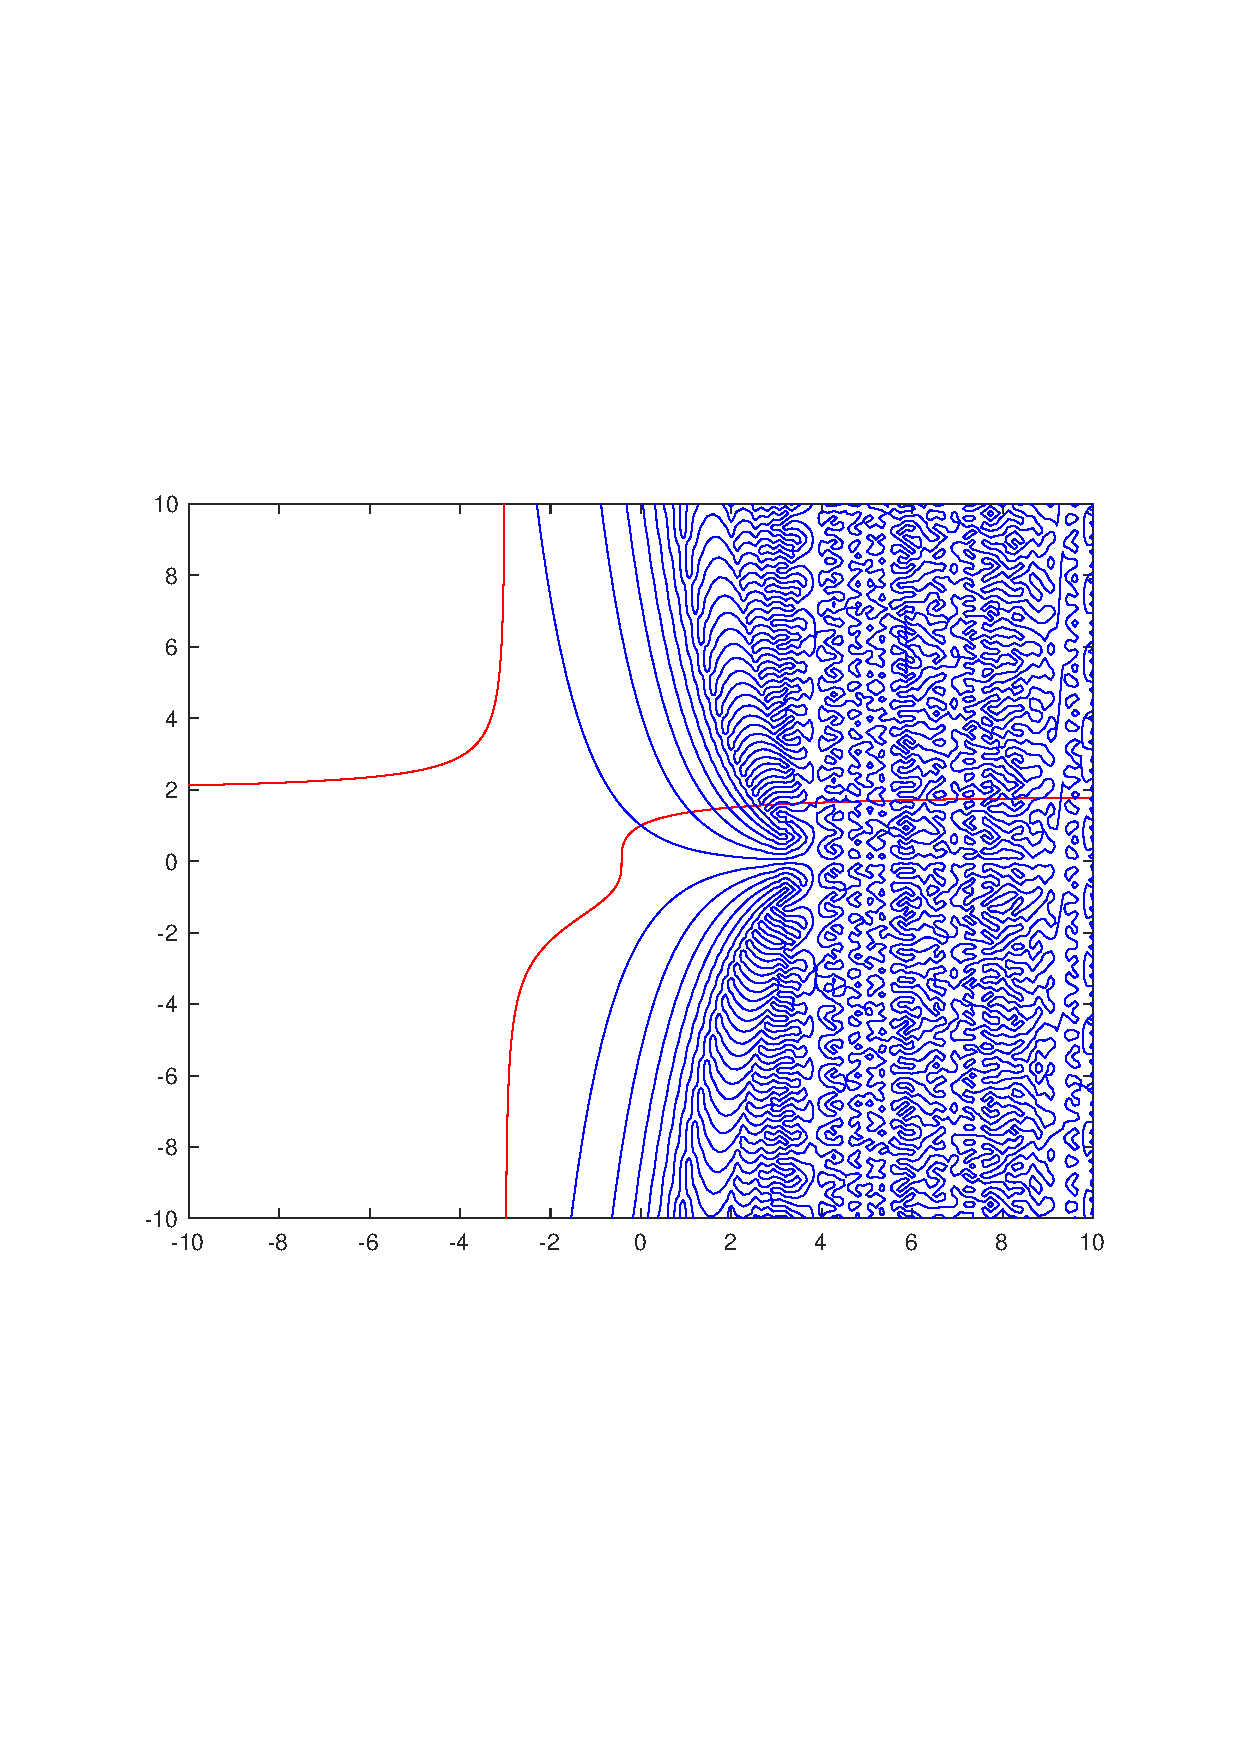
\includegraphics[scale=0.65]{image/MATLAB.pdf}
  \caption{{M\footnotesize{ATLAB}}绘制方程组\eqref{eq:11}图像的示意图}
  \label{pic:1}
\end{figure}\par
图\ref{pic:1}的绘制采用如下的M{\footnotesize{ATLAB}}代码:
\begin{Matlab}
  f=@(x,y) (x+3)*(y^3-7)+18;
  fimplicit(f,[-10 25 -10 25],'r') 

  hold on

  g=@(x,y) sin(y*exp(x)-1);
  fimplicit(g,[-10 25 -10 25],'b')

  hold off
\end{Matlab}\newpage\par
在Python 3.7.7中利用\tcbox{matplotlib}和\tcbox{numpy}绘制的方程组\eqref{eq:11}图像如图\ref{pic:2}所示:
\begin{figure}[H]
  \centering
  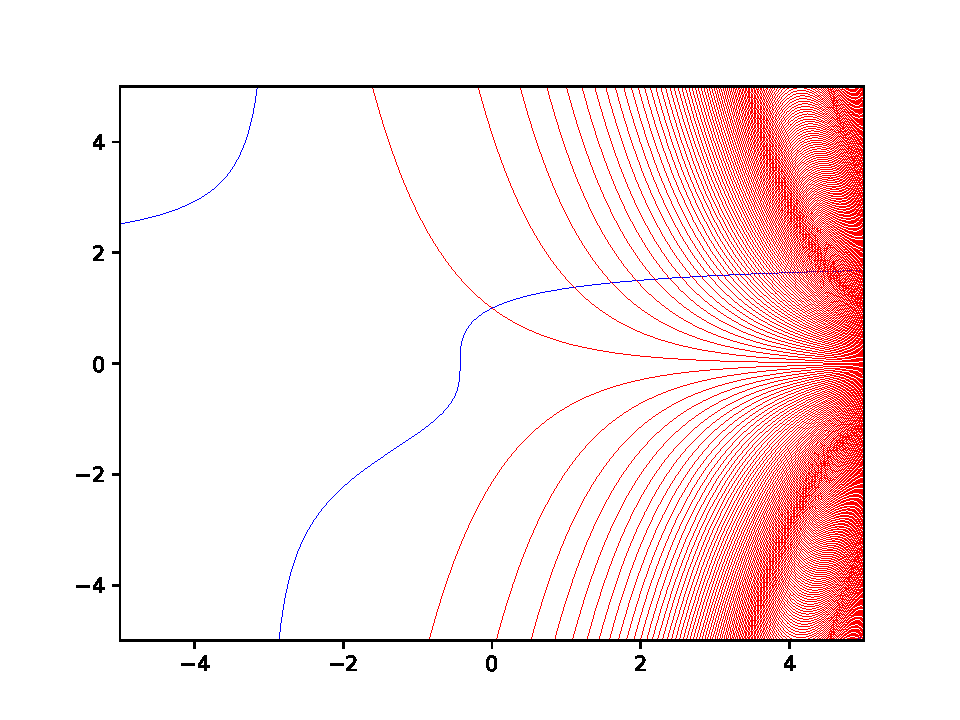
\includegraphics[scale=0.80]{image/Python.pdf}
  \caption{Python绘制方程组\eqref{eq:11}图像的示意图}
  \label{pic:2}
\end{figure}\par
图\ref{pic:2}的绘制采用如下的Python代码:
\begin{Python}
  import matplotlib.pyplot as plt
  import numpy as np
  
  def f(x,y):
      return (x+3)*(y**3-7)+18
  def g(x,y):
      return np.sin(y*np.exp(x)-1)
  
  n=500
  x=np.linspace(-5,5,500)
  y=np.linspace(-5,5,500)
  
  X,Y=np.meshgrid(x,y)
  
  plt.contour(X,Y,f(X,Y),1,colors='b',linewidths=0.4)    
  plt.contour(X,Y,g(X,Y),1,colors='r',linewidths=0.4)
  
  plt.show()
\end{Python}\par
根据图\ref{pic:1}和图\ref{pic:2}的结果,选取交点附近的坐标值作为初始值进行迭代. 采用如下的{M\footnotesize{ATLAB}}代码对方程组\eqref{eq:11}交点附近的值进行牛顿迭代.\newpage\par
子程序一\tcbox{F.m}用于求每一步的\(\b{F}(\b{x})\).  
\begin{Matlab}
  function[out]=F(x,y)
  syms x1 x2;
  f1=(x1+3)*(x2^3-7)+18;
  f2=sin(x2*exp(x1)-1);
  Y=[f1;f2];
  x1=x;
  x2=y;
  out=subs(Y);
  end
\end{Matlab}\par
子程序二\tcbox{JF.m}用于求每一步的雅克比矩阵.
\begin{Matlab}
  function[y]=JF(x,y)
  syms x1 x2
  f1=(x1+3)*(x2^3-7)+18;
  f2=sin(x2*exp(x1)-1);
  df1x=diff(sym(f1),'x1');
  df1y=diff(sym(f1),'x2');
  df2x=diff(sym(f2),'x1');
  df2y=diff(sym(f2),'x2');
  j=[df1x,df1y;df2x,df2y];
  x1=x;
  x2=y;
  y=double(subs(j));
  end
\end{Matlab}\par
主程序\tcbox{Newton.m}是对方程组\eqref{eq:11}进行牛顿迭代.
\begin{Matlab}
  function[Z,P,k,E,S]=Newton(P,e0)
  Z=F(P(1),P(2));
  J=JF(P(1),P(2));
  Q=P-J\Z;
  e=norm((Q-P),inf);
  P=Q;
  Z=F(P(1),P(2));
  S=[Q];
  E=[e];
  k=1;
  while e>=e0
     J=JF(P(1),P(2));
     Q=P-J\Z;
     e=norm((Q-P),inf);
     P=Q;
     Z=F(P(1),P(2));
     S=[S P];
     E=[E e];
     k=k+1;
  end
  Z=vpa(Z)
  P=vpa(P);
  S=vpa(S);
  E=vpa(E);
  end
\end{Matlab}\par
设置精度为\(\b{e}=10^{-5}\),在{M\footnotesize{ATLAB}} R2020a分别取如表\ref{tab}所示的初始值运行程序\tcbox{F.m}、\tcbox{JF.m}和\tcbox{Newton.m}. 并得到接下来的六组迭代结果:
\begin{table}[H]
  \centering
  \caption{\(6\)次迭代选取的初始值}
  \label{tab}
  \begin{NiceTabular}{ccccccc}
    \toprule[1pt]
    迭代结果 & 表\ref{tab:1} & 表\ref{tab:2} & 表\ref{tab:3} & 表\ref{tab:4} & 表\ref{tab:5} & 表\ref{tab:6}\\
    \midrule[0.8pt]
    \makecell[c]{迭代初始值\\ \(\big(\b{x}_1^0,\b{x}_2^0\big)\)} & \makecell[c]{-0.040\\0.96} & \makecell[c]{1.075\\1.34} & \makecell[c]{1.604\\1.42} & \makecell[c]{1.935\\1.46} & \makecell[c]{2.177\\1.49} & \makecell[c]{2.688\\1.54}\\
    \bottomrule[1pt]
  \end{NiceTabular}
\end{table}

\begin{table}[H]
  \centering
  \caption{初始值为\((-0.040,0.96)\)的迭代结果}
  \label{tab:1}
  \begin{NiceTabular}{cccc}[code-before=\rowcolor{red!15}{1}\rowcolors{2}{blue!15}{}]
    \toprule[1pt]
    迭代次数 & \(\b{x}_1\) & \(\b{x}_2\) &\(\b{e}\)\\
    \midrule[0.8pt]
    1 & \makecell[l]{0.00018764791983762\\444721611681478909} & \makecell[l]{1.002393408614774\\1826527201579592} & \makecell[l]{0.0423934086147741\\82652720157959161}\\
    2 & \makecell[l]{-0.00000324227614454\\1249896480214001084} & \makecell[l]{1.00000371102556\\48227175119899779} & \makecell[l]{0.0023896975892093\\599352081679812331}\\
    3 & \makecell[l]{-0.00000000000992216042\\57619582046569943993453} & \makecell[l]{1.000000000003146\\2105318997286378} & \makecell[l]{0.000003711022418612\\1856122613401583001}\\
    \bottomrule[1pt]
  \end{NiceTabular} 
\end{table} 

\begin{table}[H]
  \centering
  \caption{初始值为\((1.075,1.34)\)的迭代结果}
  \label{tab:2}
  \begin{NiceTabular}{cccc}[code-before=\rowcolor{red!15}{1}\rowcolors{2}{blue!15}{}]
    \toprule[1pt]
    迭代次数 & \(\b{x}_1\) & \(\b{x}_2\) &\(\b{e}\)\\
    \midrule[0.8pt]
    1 & \makecell[l]{1.102024869036446\\6056395111699049} & \makecell[l]{1.378461462387132\\9155940821227552} & \makecell[l]{0.0384614623871329\\15594082122755166}\\
    2 & \makecell[l]{1.101168345107749\\7215327639922375} & \makecell[l]{1.377008371470982\\9065809546580189} & \makecell[l]{0.0014530909161500\\090131274647362467}\\
    3 & \makecell[l]{1.101168436301883\\0651330315890114} & \makecell[l]{1.377006550054511\\0421307263105578} & \makecell[l]{0.000001821416471864\\4502283474611172107}\\
    \bottomrule[1pt]
  \end{NiceTabular} 
\end{table} 

\begin{table}[H]
  \centering
  \caption{初始值为\((1.604,1.42)\)的迭代结果}
  \label{tab:3}
  \begin{NiceTabular}{cccc}[code-before=\rowcolor{red!15}{1}\rowcolors{2}{blue!15}{}]
    \toprule[1pt]
    迭代次数 & \(\b{x}_1\) & \(\b{x}_2\) &\(\b{e}\)\\
    \midrule[0.8pt]
    1 & \makecell[l]{1.608964997342521\\8249898739813013} & \makecell[l]{1.458274363802354\\2205596517677181} & \makecell[l]{0.0382743638023542\\20559651767718068}\\
    2 & \makecell[l]{1.609013900511893\\8845434633231169} & \makecell[l]{1.457254768660919\\1167963985250797} & \makecell[l]{0.0010195951414351\\037632532426383762}\\
    3 & \makecell[l]{1.609014377222653\\6136092463460571} & \makecell[l]{1.457254129187330\\5584033693427254} & \makecell[l]{0.000000639473588558\\39302918235430635174}\\
    \bottomrule[1pt]
  \end{NiceTabular} 
\end{table}

\begin{table}[H]
  \centering
  \caption{初始值为\((1.935,1.46)\)的迭代结果}
  \label{tab:4}
  \begin{NiceTabular}{cccc}[code-before=\rowcolor{red!15}{1}\rowcolors{2}{blue!15}{}]
    \toprule[1pt]
    迭代次数 & \(\b{x}_1\) & \(\b{x}_2\) &\(\b{e}\)\\
    \midrule[0.8pt]
    1 & \makecell[l]{1.941043297812879\\3617050840017134} & \makecell[l]{1.498344996495315\\1981785313276591} & \makecell[l]{0.0383449964953151\\98178531327659099}\\
    2 & \makecell[l]{1.940535487293205\\9732938724667489} & \makecell[l]{1.497280415079132\\5703198137357562} & \makecell[l]{0.0010645814161826\\278587175919028949}\\
    3 & \makecell[l]{1.940535631232127\\7062195660593209} & \makecell[l]{1.497279563996578\\3454833642453727} & \makecell[l]{0.000000851082554224\\83644949038346122073}\\
    \bottomrule[1pt]
  \end{NiceTabular} 
\end{table}

\begin{table}[H]
  \centering
  \caption{初始值为\((2.177,1.49)\)的迭代结果}
  \label{tab:5}
  \begin{NiceTabular}{cccc}[code-before=\rowcolor{red!15}{1}\rowcolors{2}{blue!15}{}]
    \toprule[1pt]
    迭代次数 & \(\b{x}_1\) & \(\b{x}_2\) &\(\b{e}\)\\
    \midrule[0.8pt]
    1 & \makecell[l]{2.188893030333566\\2304580607740597} & \makecell[l]{1.523574396024620\\5541318038807763} & \makecell[l]{0.0335743960246205\\54131803880776286}\\
    2 & \makecell[l]{2.187171863987524\\6189111099797759} & \makecell[l]{1.522606834111617\\4938342254789248} & \makecell[l]{0.0017211663460416\\115469507942837653}\\
    3 & \makecell[l]{2.18717077695660\\865007833770624} & \makecell[l]{1.522605792985845\\9530825293565194} & \makecell[l]{0.000001087030915968\\8327722735358985321}\\
    \bottomrule[1pt]
  \end{NiceTabular} 
\end{table}

\begin{table}[H]
  \centering
  \caption{初始值为\((2.688,1.54)\)的迭代结果}
  \label{tab:6}
  \begin{NiceTabular}{cccc}[code-before=\rowcolor{red!15}{1}\rowcolors{2}{blue!15}{}]
    \toprule[1pt]
    迭代次数 & \(\b{x}_1\) & \(\b{x}_2\) &\(\b{e}\)\\
    \midrule[0.8pt]
    1 & \makecell[l]{2.687419770586015\\9720618844782872} & \makecell[l]{1.565698197765964\\7484947454132387} & \makecell[l]{0.0256981977659647\\48494745413238669}\\
    2 & \makecell[l]{2.687059806168365\\8036809129748115} & \makecell[l]{1.565256347405070\\1238022869460335} & \makecell[l]{0.00044185036089462\\469245846720520842}\\
    3 & \makecell[l]{2.687059785059851\\0707426894123864} & \makecell[l]{1.565256193072133\\7807870572778944} & \makecell[l]{0.000000154332936343\\01522966813907154719}\\
    \bottomrule[1pt]
  \end{NiceTabular} 
\end{table}\par
观察图\ref{pic:1}和图\ref{pic:2},我们可以发现在\(y\)轴正方向可能会有交点,因此我们选取区域\([-5,0]\times[15,25]\)分别采用{M\footnotesize{ATLAB}}和Python作出方程组\eqref{eq:11}在此区域的图像如图\ref{pic:3}所示.
\begin{figure}[H]
  \centering
  \subfigure[{M\scriptsize{ATLAB}}绘制的图像]{
      \begin{minipage}[t]{7.0cm}
          \centering
          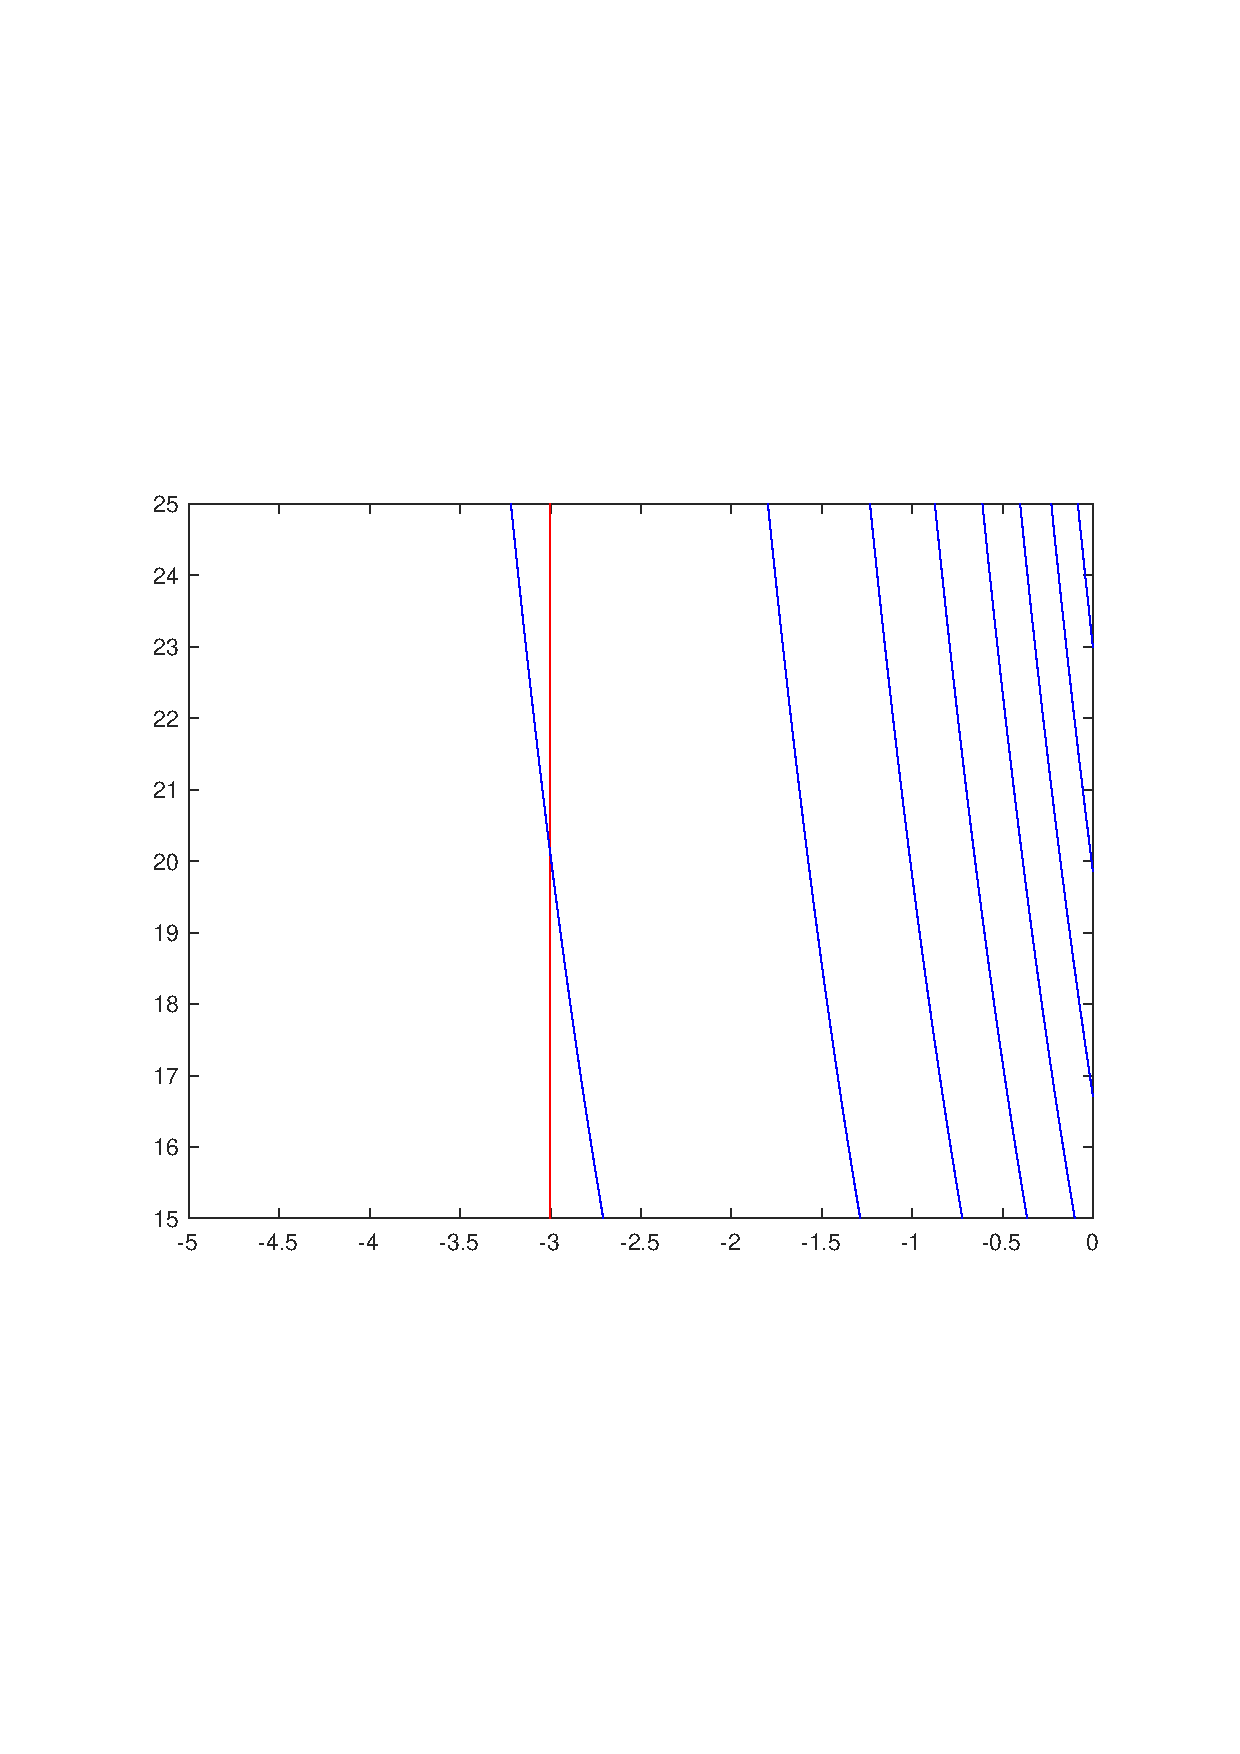
\includegraphics[scale=0.400]{image/MATLAB_1.pdf}
      \end{minipage}
  }    
  \subfigure[Python绘制的图像]{
      \begin{minipage}[t]{7.0cm}
          \centering
          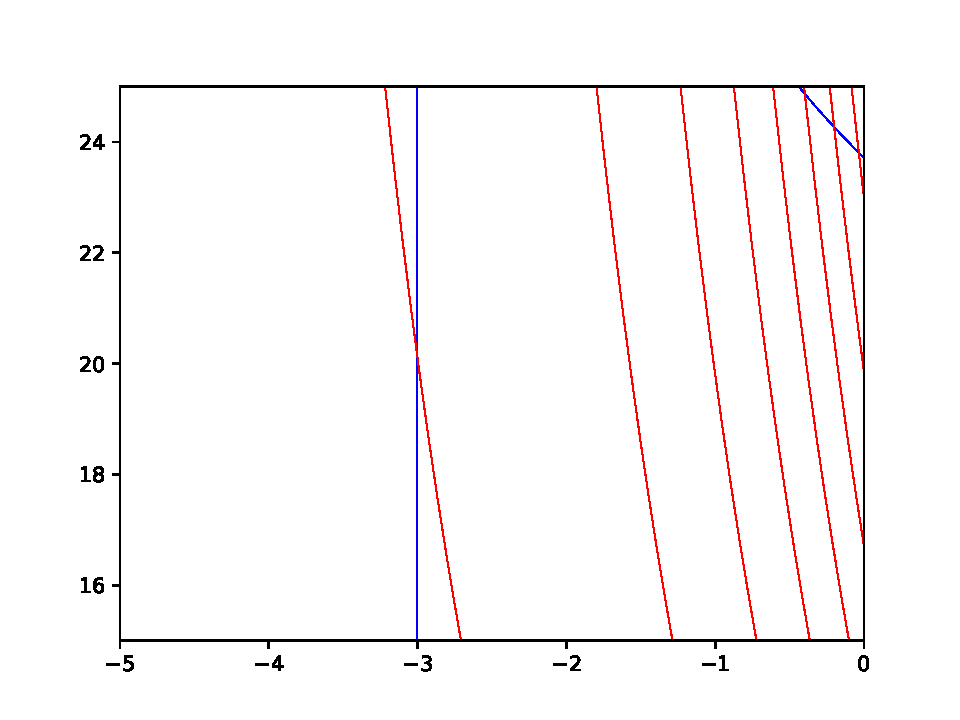
\includegraphics[scale=0.512]{image/Python_1.pdf}
      \end{minipage}
  }
  \caption{方程组\eqref{eq:11}在点\((-3.006,20.23)\)附近的交点示意图}
  \label{pic:3}
\end{figure}\par
根据图\ref{pic:3}所示,我们可以看出在区域\([-5,0]\times[15,25]\)方程组\eqref{eq:11}的确有交点,选取\((-3.006,20.23)\)作为初始值进行迭代,有如下的迭代结果:
\begin{table}[H]
  \centering
  \caption{初始值为\((-3.006,20.23)\)的迭代结果}
  \label{tab:7}
  \begin{NiceTabular}{cccc}[code-before=\rowcolor{red!15}{1}\rowcolors{2}{blue!15}{}]
    \toprule[1pt]
    迭代次数 & \(\b{x}_1\) & \(\b{x}_2\) &\(\b{e}\)\\
    \midrule[0.8pt]
    1 & \makecell[l]{-3.00226427175802\\79666497409029065} & \makecell[l]{20.13083861550757\\5239629863760843} & \makecell[l]{0.0991613844924247\\60370136239157416}\\
    2 & \makecell[l]{-3.00220860943217\\44145494655474207} & \makecell[l]{20.12994703530901\\7541420661938202} & \makecell[l]{0.00089158019855769\\820920182264087115}\\
    3 & \makecell[l]{-3.00220860205891\\79266550165537932} & \makecell[l]{20.12994690532731\\5207307796741835} & \makecell[l]{0.000000129981702334\\11286519636643249399}\\
    \bottomrule[1pt]
  \end{NiceTabular} 
\end{table}

\section{牛顿迭代法的优缺点}
牛顿迭代法是梯度下降法的进一步发展,梯度下降法以目标函数的一阶偏导数作为信息、以负梯度方向作为搜索方向,只考虑目标函数在迭代点的局部性质;而牛顿迭代法不仅使用目标函数的一阶偏导数,而且进一步利用目标函数的二阶偏导数,考虑了梯度变化的趋势,因而能更全面地确定合适的搜索方向加快收敛.\par
但牛顿迭代法存在以下两个缺点:
\begin{enumerate}
  \item 对目标函数有较严格的要求. 函数必须具有连续的一、二阶偏导数,黑塞矩阵必须正定.
  \item 计算复杂,除需计算梯度外,仍需计算雅可比矩阵及其逆矩阵. 计算量、存储量均很大,且均以维数\(n\)的平方增加,当\(n\)很大时问题更加突出.
\end{enumerate}\par
为了克服上述问题,人们提出了\emph{拟牛顿法}. 此方法的基本思想是: 不用二阶偏导数而构造出近似的正定对称的黑塞矩阵或黑塞矩阵的逆矩阵,在拟牛顿的条件下优化目标函数. 不同的构造方法会产生不同的拟牛顿法. 即对算法中用来计算搜索方向的黑塞矩阵或黑塞矩阵的逆矩阵作近似计算.


\nocite{*}
\bibliography{wpref}

\end{document}
